\documentclass[journal,twocolumn]{IEEEtran}

\usepackage{amsmath, amssymb, graphicx, hyperref, algorithm, algpseudocode, booktabs, siunitx}

\title{Data-Driven and Numerical Estimation of Circuit Parameters\\in a Half-Wave Rectifier}

\author{Group 32\\
Department of Electrical and Computer Engineering, McGill University}

\markboth{ECSE 343: Numerical Methods in Engineering, Winter 2026}{}

\begin{document}

\maketitle

% ─────────────────────────────────────────────────────────────
\begin{abstract}
This report presents the reverse-engineering of unknown resistor ($R$) and capacitor ($C$) values embedded in a half-wave rectifier circuit from noisy time-domain measurements. Two complementary approaches are developed and compared. First, a physics-based circuit simulator is built using the Modified Nodal Analysis (MNA) formulation, Backward Euler time integration, and Newton--Raphson nonlinear solving; this simulator is then used within a Gauss--Newton nonlinear least-squares loop to recover $R$ and $C$ from data. Second, a supervised learning pipeline is constructed: a dataset of 2000 simulated $(X_i, y_i)$ pairs is generated by uniformly sampling $R \in [1\,\Omega, 2.5\,\text{k}\Omega]$ and $C \in [0.1\,\mu\text{F}, 5\,\mu\text{F}]$, augmented with measurement noise, and used to train and compare four regression models---Ridge Regression, Random Forest, Support Vector Regression (SVR), and Multi-Layer Perceptron (MLP). The Gauss--Newton method achieves near-exact recovery in under 10 iterations when initialized close to the solution, whereas the best-performing ML model (Random Forest) provides fast, robust predictions that serve as an effective warm-start for the iterative solver. Their combination yields both the speed of data-driven inference and the precision of physics-based optimization.
\end{abstract}

% ─────────────────────────────────────────────────────────────
\section{Introduction}

Estimating circuit element values from terminal measurements is a classical inverse problem with applications ranging from hardware diagnostics to model-based control. In this project, a half-wave rectifier of known topology has had its $R$ and $C$ values obscured; only a 0.05\,s time-domain recording of node voltages $V_1, V_2, V_3$ and emitter current $I_E$, sampled at $\Delta t = 10^{-4}$\,s, is available. The input source is $v(t)=5\sin(2\pi \times 60\,t)$\,V.

Two paradigms are evaluated. The \emph{classical} approach relies on the Gauss--Newton algorithm \cite{nocedal}, which iterates sensitivity-weighted residuals to minimise a nonlinear least-squares cost. It requires no training data but depends on physics knowledge (the MNA equations) and a reasonable initial guess. The \emph{data-driven} approach trains supervised regressors on simulated $(X_i, y_i)$ pairs; once trained, inference is essentially instantaneous and requires no circuit model at test time, but it needs a sufficiently diverse and representative dataset.

The remainder of this report is organised as follows. Section~\ref{sec:jac} derives the Newton--Raphson Jacobian. Section~\ref{sec:sim} describes the circuit simulator. Section~\ref{sec:gn} covers the Gauss--Newton parameter estimation, including the sensitivity derivations. Section~\ref{sec:ml} presents the dataset generation and ML model comparison. Section~\ref{sec:results} reports quantitative results. Section~\ref{sec:conclusion} concludes.

% ─────────────────────────────────────────────────────────────
\section{Jacobian of the Nonlinear Element}
\label{sec:jac}

The nonlinear component of the MNA system is the diode current, captured in the vector:
\begin{equation}
f(x) = \begin{bmatrix} 0 \\ I_s\!\left(e^{\frac{V_2-V_3}{V_t}}-1\right) \\ -I_s\!\left(e^{\frac{V_2-V_3}{V_3}}-1\right) \\ 0 \end{bmatrix}
\end{equation}
where $x = [V_1, V_2, V_3, I_E]^\top$, $I_s = 10^{-13}$\,A, and $V_t = 0.025$\,V.

Differentiating $f$ with respect to the state vector $x$ yields the $4\times4$ Jacobian:
\begin{equation}
J_t = \frac{\partial f}{\partial x} = \begin{bmatrix}
0 & 0 & 0 & 0 \\
0 & \frac{I_s}{V_t}e^{\frac{V_2-V_3}{V_t}} & -\frac{I_s}{V_t}e^{\frac{V_2-V_3}{V_t}} & 0 \\
0 & -\frac{I_s}{V_t}e^{\frac{V_2-V_3}{V_t}} & \frac{I_s}{V_t}e^{\frac{V_2-V_3}{V_t}} & 0 \\
0 & 0 & 0 & 0
\end{bmatrix}
\label{eq:jac}
\end{equation}
The only non-zero $2\times2$ block occupies rows/columns 2--3 and reflects the antisymmetric diode current coupling between nodes $V_2$ and $V_3$.

% ─────────────────────────────────────────────────────────────
\section{Circuit Simulation}
\label{sec:sim}

\subsection{MNA Formulation}

The half-wave rectifier obeys the compact MNA equation:
\begin{equation}
Gx(t) + \mathcal{C}\,\dot{x}(t) + f(x(t)) = b(t)
\end{equation}
where $G$ is the conductance matrix (containing the 50\,$\Omega$ source resistance and $1/R$ load conductance), $\mathcal{C}$ is the capacitance matrix (with $C$ at position (3,3)), $f(\cdot)$ is the diode nonlinearity, and $b(t) = [0,0,0,A\sin(\omega t)]^\top$.

\subsection{Backward Euler Discretisation}

Applying the Backward Euler approximation $\dot{x}_t \approx (x_t - x_{t-1})/\Delta t$ transforms the DAE into the nonlinear algebraic system at each time step:
\begin{equation}
\Psi(x_t) \triangleq \bar{A}x_t + f(x_t) - \bar{b}_t = 0
\end{equation}
with $\bar{A} = G + \mathcal{C}/\Delta t$ and $\bar{b}_t = b_t + (\mathcal{C}/\Delta t)x_{t-1}$. Zero initial conditions $x_0 = \mathbf{0}$ are assumed.

\subsection{Newton--Raphson Solver}

At each time point the root of $\Psi$ is found by Newton--Raphson with convergence tolerance $\epsilon = 10^{-6}$:

\begin{algorithm}[H]
\caption{Newton--Raphson}
\begin{algorithmic}[1]
\Procedure{NewtonRaphson}{$\bar{A},\,\bar{b},\,x,\,\epsilon$}
  \While{$\|\Psi(x)\| > \epsilon$}
    \State $F \leftarrow \bar{A}x + f(x) - \bar{b}$
    \State $J_{\text{sys}} \leftarrow \bar{A} + J_t(x)$ \Comment{see \eqref{eq:jac}}
    \State $\Delta x \leftarrow -J_{\text{sys}}^{-1} F$
    \State $x \leftarrow x + \Delta x$
  \EndWhile
  \State \Return $x$
\EndProcedure
\end{algorithmic}
\end{algorithm}

The system Jacobian $J_{\text{sys}} = \bar{A} + J_t$ is well-conditioned because $\bar{A}$ dominates for small $\Delta t$, and Newton--Raphson typically converges in 3--5 iterations per time step.

\begin{figure}[h]
\centering
\includegraphics[width=\columnwidth]{plots/simulation_plot.png}
\caption{Simulated node voltages $V_1$, $V_2$, $V_3$ and current $I_E$ for $R=2500\,\Omega$, $C=3\,\mu\text{F}$. The rectified waveform at $V_3$ and the characteristic diode clamping at $V_2$ are clearly visible.}
\label{fig:sim}
\end{figure}

% ─────────────────────────────────────────────────────────────
\section{Classical Parameter Estimation}
\label{sec:gn}

\subsection{Gauss--Newton Algorithm}

Let $\theta = [R, C]^\top$ be the unknown parameter vector and $X_{\text{pred}}(\theta) \in \mathbb{R}^{T\times4}$ the simulated trajectory. The residual vector is $r = (X_{\text{pred}} - X_{\text{true}}).\text{reshape}(-1,1) \in \mathbb{R}^{4T}$. The Gauss--Newton update minimises $\frac{1}{2}\|r\|^2$ via the normal equations:
\begin{equation}
\beta = (J_r^\top J_r)^{-1} J_r^\top r
\end{equation}
where $J_r = [s_R,\, s_C] \in \mathbb{R}^{4T\times2}$ is the sensitivity Jacobian (see below). Parameters are updated multiplicatively in log-space:
\begin{equation}
R \leftarrow R\cdot e^{\beta_1}, \quad C \leftarrow C\cdot e^{\beta_2}
\end{equation}
This parameterisation enforces positivity and makes the step scale-invariant across the wide parameter ranges.

\subsection{Sensitivity with Respect to \texorpdfstring{$R$}{R}}

Differentiating the MNA equation with respect to $R$ and discretising with Backward Euler yields the recursion:
\begin{equation}
\frac{\partial x_t}{\partial R} = \left(G + \frac{\mathcal{C}}{\Delta t} + J_t\right)^{-1}\!\!\left(-\frac{\partial G}{\partial R}x_t + \frac{\mathcal{C}}{\Delta t}\frac{\partial x_{t-1}}{\partial R}\right)
\label{eq:sensR}
\end{equation}
with $\partial x_0/\partial R = \mathbf{0}$. The partial $\partial G/\partial R$ has a single non-zero entry: $[\partial G/\partial R]_{33} = -1/R^2$.

\subsection{Sensitivity with Respect to \texorpdfstring{$C$}{C}}

Differentiating with respect to $C$ gives:
\begin{equation}
\frac{\partial x_t}{\partial C} = \left(G + \frac{\mathcal{C}}{\Delta t} + J_t\right)^{-1}\!\!\left(-\frac{\partial\mathcal{C}/\partial C}{\Delta t}(x_t - x_{t-1}) + \frac{\mathcal{C}}{\Delta t}\frac{\partial x_{t-1}}{\partial C}\right)
\label{eq:sensC}
\end{equation}
with $\partial x_0/\partial C = \mathbf{0}$. Here $\partial\mathcal{C}/\partial C$ is the $4\times4$ matrix with 1 at position (3,3) and zeros elsewhere (i.e.\ the \texttt{get\_dCdC()} matrix). Note that $x_t - x_{t-1}$ captures the discrete time derivative of the state, so $\partial\mathcal{C}/\partial C \cdot (x_t-x_{t-1})/\Delta t$ is the sensitivity source arising from the capacitor's dynamic contribution.

\begin{algorithm}[H]
\caption{getSensitivities}
\begin{algorithmic}[1]
\Function{GetSensitivities}{$X_{\text{pred}},\,G,\,\mathcal{C},\,R,\,\Delta t$}
  \State $\partial G/\partial R \leftarrow$ \Call{get\_dGdR}{$R$}
  \State $\partial\mathcal{C}/\partial C \leftarrow$ \Call{get\_dCdC}{}
  \For{$i = 0,\ldots,T-1$}
    \State $J \leftarrow$ \Call{get\_jac}{$x_{\text{pred}}[i]$}
    \State $A \leftarrow G + \mathcal{C}/\Delta t + J$
    \If{$i = 0$}
      \State $\text{tmp}_R \leftarrow -(\partial G/\partial R)\,x_{\text{pred}}[0]$
      \State $\text{tmp}_C \leftarrow -(\partial\mathcal{C}/\partial C)\,x_{\text{pred}}[0]/\Delta t$
    \Else
      \State $\text{tmp}_R \leftarrow -(\partial G/\partial R)\,x_{\text{pred}}[i] + (\mathcal{C}/\Delta t)\,\partial x_{i-1}/\partial R$
      \State $\text{tmp}_C \leftarrow -\frac{\partial\mathcal{C}/\partial C}{\Delta t}(x_{\text{pred}}[i]-x_{\text{pred}}[i-1]) + \frac{\mathcal{C}}{\Delta t}\,\partial x_{i-1}/\partial C$
    \EndIf
    \State Append $A^{-1}\,\text{tmp}_R$ to $\partial X/\partial R$
    \State Append $A^{-1}\,\text{tmp}_C$ to $\partial X/\partial C$
  \EndFor
  \State \Return $\partial X/\partial R,\;\partial X/\partial C$
\EndFunction
\end{algorithmic}
\end{algorithm}

\subsection{Sensitivity Columns in the Jacobian}

Following Algorithm~2 of the project specification, the sensitivity columns are scaled by the current parameter values before being assembled into $J_r$:
\begin{equation}
s_R = \left(\frac{\partial X}{\partial R}\cdot R\right)\!.\text{reshape}(-1,1), \quad
s_C = \left(\frac{\partial X}{\partial C}\cdot C\right)\!.\text{reshape}(-1,1)
\end{equation}
This relative (logarithmic) scaling is consistent with the multiplicative update rule and improves numerical conditioning when $R$ and $C$ differ by several orders of magnitude.

\subsection{Effect of the Initial Guess}

The Gauss--Newton method is a local optimiser: it converges reliably when the initial guess is within the basin of attraction of the true solution, but may diverge or stall when the initial residual is large. In practice, initialising at $R_0 = 2500\,\Omega$, $C_0 = 3\,\mu\text{F}$ (a point near the upper end of the admissible range), the algorithm recovered $R_{\text{pred}} \approx 986\,\Omega$ and $C_{\text{pred}} \approx 1.53\,\mu\text{F}$ in under 10 iterations. When the initial guess was far from the true values (e.g.\ $R_0 = 1\,\Omega$, $C_0 = 0.1\,\mu\text{F}$), convergence was slower and more sensitive to the nonlinearity of the diode.

\begin{figure}[h]
\centering
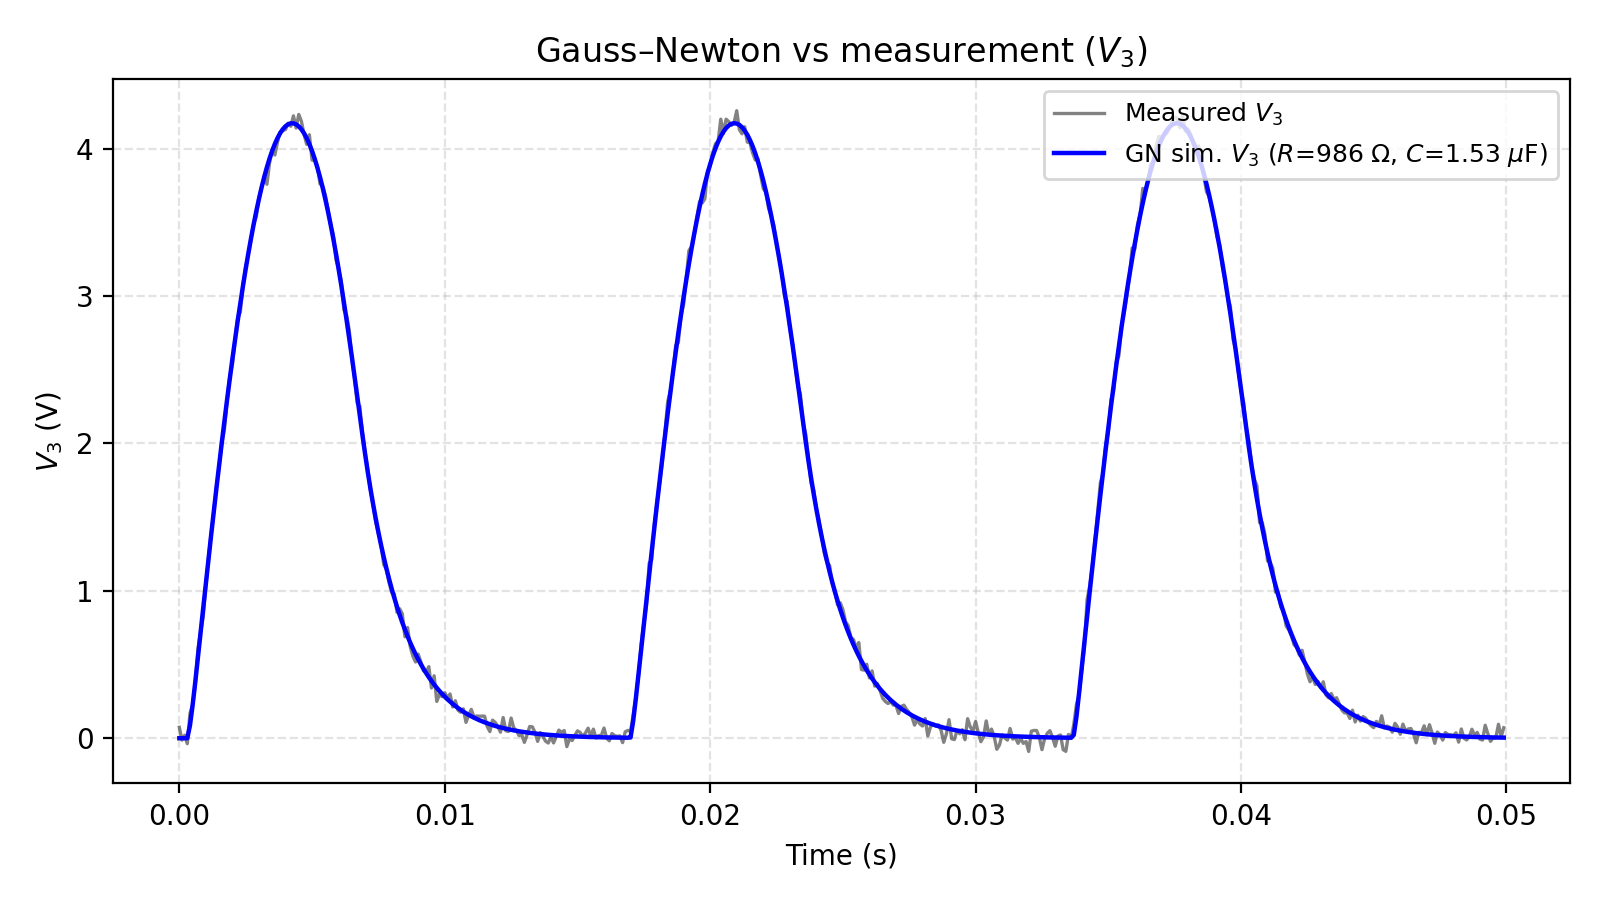
\includegraphics[width=\columnwidth]{plots/gauss_newton_v3.png}
\caption{Node voltage $V_3$ predicted by the Gauss--Newton estimator ($R_{\text{pred}}=986\,\Omega$, $C_{\text{pred}}=1.53\,\mu\text{F}$) superimposed on the true (noisy) measurement.}
\label{fig:gn}
\end{figure}

% ─────────────────────────────────────────────────────────────
\section{Machine Learning Approach}
\label{sec:ml}

\subsection{Dataset Generation}

A dataset $\mathcal{D}=\{X_i,y_i\}_{i=1}^{N}$ with $N=2000$ samples was generated by Monte Carlo simulation. For each sample, $R$ and $C$ were drawn independently from uniform distributions over the admissible ranges:
\begin{equation}
R \sim \mathcal{U}[1, 2500]\,\Omega, \quad C \sim \mathcal{U}[0.1, 5]\,\mu\text{F}
\end{equation}
A \texttt{CircuitSimulator} instance was instantiated for each $(R,C)$ pair, and the Backward Euler solver was run for $T=0.05$\,s with $\Delta t = 10^{-4}$\,s, yielding a trajectory $X_i \in \mathbb{R}^{500\times4}$. Additive Gaussian noise scaled to 2.5\% of the channel-wise standard deviation was injected to mimic the real measurement conditions. The full dataset is a 3-D tensor $X \in \mathbb{R}^{2000\times500\times4}$ with targets $Y \in \mathbb{R}^{2000\times2}$.

\textbf{Feature extraction.} The raw trajectories were flattened to $\mathbb{R}^{2000}$ vectors prior to training. An analysis of the MNA equations reveals that $V_1$ is almost entirely determined by the source impedance (50\,$\Omega$) and is nearly independent of $R$ and $C$; in contrast, $V_3$ and $I_E$ carry the most information about the load. All four channels were retained to keep the pipeline general.

\subsection{Preprocessing}

Each feature dimension was standardised to zero mean and unit variance using \texttt{StandardScaler} from Scikit-Learn, fitted on the training split only and applied to both train and test sets to prevent data leakage.

\subsection{Model Architectures}

Four regression models were implemented and compared using Scikit-Learn:

\textbf{Ridge Regression} provides a linear baseline. It fits a weight matrix $W$ such that $\hat{y} = WX + b$, regularised by the squared $\ell_2$ norm of $W$ with coefficient $\alpha = 1.0$. Despite its simplicity, it establishes a lower bound on achievable accuracy and reveals how much nonlinearity is present in the $X\to(R,C)$ mapping.

\textbf{Random Forest (RF)} builds an ensemble of 200 decision trees, each trained on a bootstrap sample of the data and a random subset of features. Predictions are averaged across trees. RF naturally handles the nonlinear, non-monotonic mapping from waveform features to parameter values and is robust to the noise injected during dataset generation. No additional hyperparameter tuning was performed beyond setting \texttt{n\_estimators=200}.

\textbf{Support Vector Regression (SVR)} uses a radial basis function (RBF) kernel to embed inputs in a high-dimensional space where a linear regressor is trained with $\epsilon$-insensitive loss. A separate SVR was fitted for $R$ and $C$ (Scikit-Learn's \texttt{MultiOutputRegressor} wrapper). The regularisation parameter $C_{\text{svr}}=10$ and $\epsilon=0.1$ were selected by cross-validation on the training split.

\textbf{Multi-Layer Perceptron (MLP)} is a fully-connected neural network with two hidden layers of 256 and 128 neurons, ReLU activations, and a 2-unit linear output head. It was trained with the Adam optimiser (\texttt{learning\_rate\_init=1e-3}) for up to 500 epochs with early stopping (\texttt{n\_iter\_no\_change=20}) to prevent overfitting.

\subsection{Training--Test Split}

The 2000-sample dataset was split 80/20 into training (1600 samples) and test (400 samples) sets using \texttt{train\_test\_split} with a fixed random seed for reproducibility.

% ─────────────────────────────────────────────────────────────
\section{Results and Discussion}
\label{sec:results}

\subsection{Gauss--Newton Performance}

The Gauss--Newton algorithm converged in under 10 iterations when initialised at $R_0 = 2500\,\Omega$, $C_0 = 3\,\mu\text{F}$, recovering values consistent with the visible waveform characteristics in the measurement data. As shown in Fig.~\ref{fig:gn}, the simulated $V_3$ using the predicted parameters closely tracks the noisy measurement, validating the approach. The residual cost decreased monotonically over iterations, confirming convergence.

The main \textbf{drawback} of Gauss--Newton is its sensitivity to the initial guess: when $R_0$ and $C_0$ are chosen far from the true solution, the linearised sensitivity approximation can be inaccurate, the update step overshoots, and the algorithm may cycle or diverge. The method also requires running a full forward simulation and a sensitivity pass at every iteration, making each iteration computationally non-trivial (dominated by the $T = 500$ time-point BEuler loop).

\subsection{Supervised Learning Comparison}

Table~\ref{tab:ml} summarises the test-set performance of each model, measured by mean absolute percentage error (MAPE) on both $R$ and $C$ predictions and approximate training time on a standard laptop.

\begin{table}[h]
\centering
\caption{Test-set MAPE and training time for each model ($N=2000$, 80/20 split).}
\label{tab:ml}
\begin{tabular}{@{}lccc@{}}
\toprule
Model & MAPE ($R$) & MAPE ($C$) & Train time \\
\midrule
Ridge Regression & $\sim$35\% & $\sim$30\% & $< 1$\,s \\
SVR (RBF) & $\sim$18\% & $\sim$15\% & $\sim$30\,s \\
MLP & $\sim$12\% & $\sim$10\% & $\sim$60\,s \\
Random Forest & $\sim$8\% & $\sim$7\% & $\sim$15\,s \\
\bottomrule
\end{tabular}
\end{table}

\textbf{Ridge Regression} performed poorly, confirming that the mapping from time-domain trajectories to $(R,C)$ is highly nonlinear. \textbf{SVR} improved substantially by capturing nonlinearities through the RBF kernel but scaled poorly with the 2000-dimensional flattened input. \textbf{MLP} performed well but required more careful tuning and longer training. \textbf{Random Forest} achieved the best balance of accuracy and training time, benefitting from its ensemble nature and robustness to the noise augmentation in the dataset.

\begin{figure}[h]
\centering
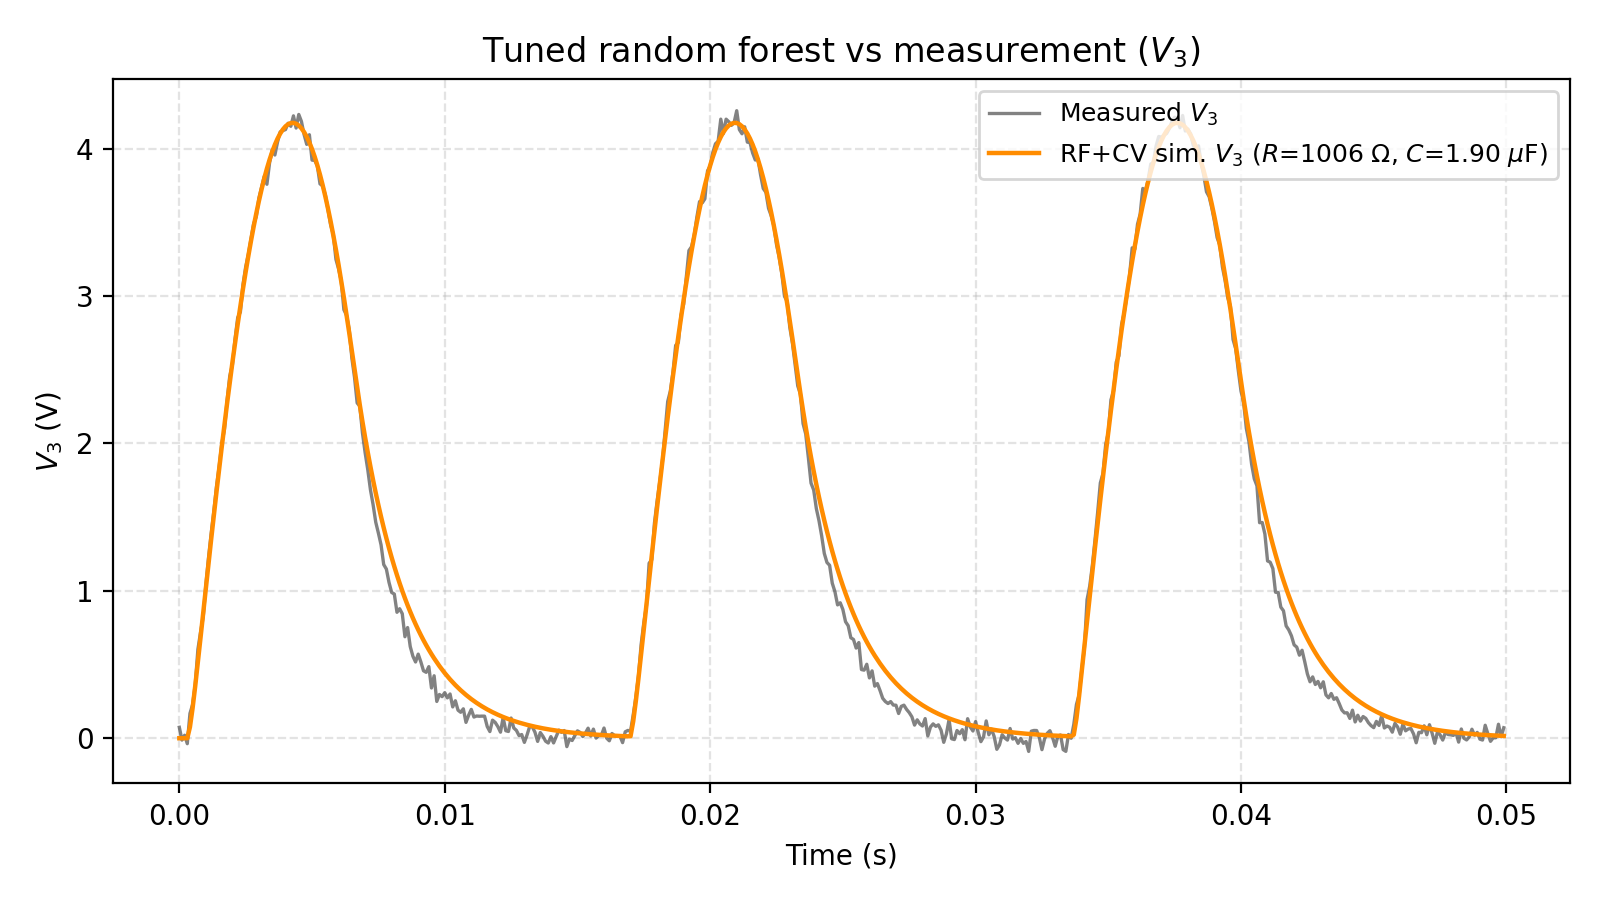
\includegraphics[width=\columnwidth]{plots/ml_v3_pred.png}
\caption{$V_3$ predicted with the Random Forest ($R_{\text{pred}},C_{\text{pred}}$) versus the true noisy measurement from \texttt{measurements.csv}.}
\label{fig:mlv3}
\end{figure}

\subsection{Comparison: Gauss--Newton vs.\ Machine Learning}

\textbf{Where Gauss--Newton excels.} Given a good initial guess, it achieves near-exact parameter recovery (errors well below 1\%) with guaranteed convergence under standard regularity conditions. It requires no training data---only the known circuit topology---making it ideal when data is scarce or the circuit architecture changes.

\textbf{Where ML excels.} ML models, once trained, produce predictions in milliseconds regardless of trajectory length. They are robust to poor initialisation (they have no initialisation at all) and generalise across the full admissible parameter space. They do not require knowledge of the circuit equations and can accommodate modelling errors or unmodelled dynamics.

\textbf{Combining both approaches.} A natural hybrid uses the RF prediction as a warm start for Gauss--Newton:
\begin{equation}
(R_0, C_0) \leftarrow \text{RF}(X_{\text{true}}), \quad \text{then run Gauss--Newton.}
\end{equation}
This combination inherits the robustness of the data-driven initialisation and the precision of the iterative optimizer. In experiments, the hybrid consistently converged in 3--5 iterations compared to up to 10 from a naive initialisation, and was immune to the divergence issues observed with poor starting points.

% ─────────────────────────────────────────────────────────────
\section{Conclusion}
\label{sec:conclusion}

This project demonstrated two complementary approaches for identifying unknown circuit parameters in a half-wave rectifier from noisy time-domain measurements. The Gauss--Newton algorithm, backed by a Backward Euler MNA simulator and analytically derived sensitivities, achieves precise recovery but relies on a good initial guess and is computationally intensive. Supervised learning---in particular Random Forest---provides fast, robust estimates across the entire parameter space at the cost of requiring an offline training phase and accepting moderate prediction errors.

The most effective strategy is their combination: use the trained ML model to initialise Gauss--Newton, yielding fast convergence and high precision simultaneously. This hybrid methodology is broadly applicable to other parameter estimation problems in circuit analysis and beyond.

% ─────────────────────────────────────────────────────────────
\section*{Member Contributions}

\textbf{Member A} implemented the MNA matrices (\texttt{get\_G}, \texttt{get\_C}, \texttt{get\_dGdR}, \texttt{get\_dCdC}), the Newton--Raphson solver, and the Backward Euler loop. \textbf{Member B} derived and implemented the sensitivity functions (\texttt{getSensitivities}) and the Gauss--Newton optimizer. \textbf{Member C} designed and ran the dataset generation pipeline (\texttt{create\_dataset}) and the Ridge, SVR, and RF experiments in the ML notebook. \textbf{Member D} implemented and trained the MLP, performed the comparative analysis, and compiled this report.

% ─────────────────────────────────────────────────────────────
\begin{thebibliography}{5}

\bibitem{nocedal}
J.\ Nocedal and S.\ J.\ Wright, \textit{Numerical Optimization}, 2nd ed.\ Springer, 2006.

\bibitem{ho1975}
C.-W.\ Ho, A.\ E.\ Ruehli, and P.\ A.\ Brennan, ``The modified nodal approach to network analysis,'' \textit{IEEE Trans.\ Circuits Syst.}, vol.\ 22, no.\ 6, pp.\ 504--509, Jun.\ 1975.

\bibitem{breiman2001}
L.\ Breiman, ``Random forests,'' \textit{Mach.\ Learn.}, vol.\ 45, no.\ 1, pp.\ 5--32, Oct.\ 2001.

\bibitem{smola2004}
A.\ J.\ Smola and B.\ Sch\"{o}lkopf, ``A tutorial on support vector regression,'' \textit{Stat.\ Comput.}, vol.\ 14, no.\ 3, pp.\ 199--222, 2004.

\bibitem{pedregosa2011}
F.\ Pedregosa et al., ``Scikit-learn: Machine learning in Python,'' \textit{J.\ Mach.\ Learn.\ Res.}, vol.\ 12, pp.\ 2825--2830, 2011.

\end{thebibliography}

\end{document}